% Kozierok, ch. 22
\chapter{IP datagram size, fragmentation, and reassembly}
\label{chap:kozierok-ch22}


The main responsibility of the Internet Protocol (IP) is to deliver data
between internetworked devices. As you saw in the preceding chapter,
this requires that data received from higher layers be encapsulated into
IP datagrams for transmission. These datagrams are then passed down to
the data link layer, where they are sent over physical network links. In
order for this to work properly, each datagram must be small enough to
fit within the frame format of the underlying technology. If the message
is bigger than the maximum frame size of the underlying network, it may
be necessary to fragment the message. The datagrams are then sent
individually and reassembled into the original message.

IP is designed to manage datagram size and to make fragmentation and
reassembly seamless. This chapter explores issues related to managing
the size of IP datagrams. I start with an overview of datagram size
issues and the important concept of a network's maximum transmission
unit (MTU), discussing why fragmentation is necessary. I then describe
the process by which messages are fragmented by the source device, and
possibly by routers along the path to the destination, and how they are
reassembled by the recipient.


\begin{backgroundinfo}
Understanding fragmentation and reassembly requires some knowledge of the basic format of IP datagrams and some of the fields they contain.
If you haven't yet read the chapter describing the general format of IP datagrams in \cref{chap:kozierok-ch21}, you may wish to review it before proceeding here.
\end{backgroundinfo}

As the core network layer protocol of the TCP/IP protocol suite, IP is designed to implement potentially large internetworks of devices.
When we work with IP, we get used to the concept of hosts being able to send information
back and forth, even though the hosts may be quite far apart. Although
we can usually consider the TCP/IP internetwork to be like a large,
abstract virtual network of devices, we must always remember that
underneath the network layer, data always travels across one or more
physical networks. The implementation of IP must take this reality into account as well.

In order to send messages using IP, we encapsulate the higher-layer data into IP datagrams.
These datagrams must then be sent down to the data link layer,
where they are further encapsulated into the frames of whatever technology will be used to physically convey them,
either directly to their destination or indirectly to the next intermediate step in their journey to their intended recipient.
The data link layer implementation puts the entire IP datagram into the data portion (the payload) of its frame format,
just as IP puts transport layer messages -- transport headers and all -- into its IP Data field.
This immediately presents us with a potential issue: matching the size of the IP datagram to the size of the underlying data link layer frame size.




\section{IP datagram size and the underlying network frame size}

The underlying network that a device uses to connect to other devices
could be a local area network (LAN) connection (like Ethernet or Token
Ring), wireless LAN (WLAN) link (such as 802.11), dial-up connection,
Digital Subscriber Line (DSL) connection, T1 link, or other wide area
network (WAN) connection. Each physical network will generally use its
own frame format, and each format has a limit on how much data can be
sent in a single frame. If the IP datagram is too large for the data
link layer frame format's payload section, we have a problem!

For example, consider an FDDI network.
The maximum size of the data field in FDDI is around 4470~bytes.
This means FDDI can handle an IP datagram of up to 4470~bytes.
In contrast, a regular Ethernet frame uses a frame format that limits the size of the payload it sends to 1500~bytes.%
\footnote{Jumbo frames support frame sizes up to about 9000~bytes.}
This means that Ethernet cannot deal with IP datagrams greater than 1500~bytes.

Now, remember that in sending a datagram across an internetwork, it may pass across more than one physical network.
To access a site on the Internet, for example, we typically send a request through our local router,
which then connects to other routers that eventually relay the request to the Internet site.
Each hop as the datagram is forwarded may use a different physical network, with a different maximum underlying frame size.

The whole idea behind a network layer protocol is to implement this concept of a virtual network where devices can communicate over great distances.
This means that higher layers shouldn't need to worry about details like the size limits of underlying data link layer technologies.
This task falls to IP.



\section{MTU and datagram fragmentation}

Each device on an IP internetwork must know the capacity of its immediate data link layer connection to other devices.
This capacity is called the \emph{maximum transmission unit} (MTU) of the network, also known as the \emph{maximum transfer unit}.

If an IP layer receives a message to be sent across the internetwork, it
looks at the size of the message and then computes how large the IP
datagram would be after the addition of the 20 or more bytes needed for
the IP header. If the total length is greater than the MTU of the
underlying network, the IP layer will fragment the message into multiple IP fragments.
Thus, if a host is connected to its local network using an Ethernet LAN, it may use an MTU of 1500~bytes for IP datagrams,
and it will fragment anything larger.

\Cref{fig:mtu-fragmentation} shows an example of different MTUs and fragmentation.


\begin{keyconcept}
The size of the largest IP datagram that can be transmitted over a physical network is called that network's \emph{maximum transmission unit} (MTU).
If a datagram is passed from a network with a high MTU to one with a low MTU, it must be fragmented to fit the other network's smaller MTU.
\end{keyconcept}

Since some physical networks on the path between devices may have a
smaller MTU than others, it may be necessary to fragment the datagram
more than once. For example, suppose the source device wants to send an
IP message 12,000 bytes long. Its local connection has an MTU of 3,300
bytes. It will need to divide this message into four fragments for
transmission: three that are about 3,300 bytes long and a fourth remnant about 2,100 bytes long.
(I'm oversimplifying by ignoring the extra headers required;
\vref{sec:ip-fragmentation-process} includes the full details of the fragmentation process.)


\begin{figure}
   \centering
   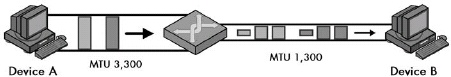
\includegraphics[width=.9\textwidth]{images/mtu-fragmentation.jpg}
   \caption
      [IP MTU and fragmentation]
      {IP maximum transmission unit (MTU) and fragmentation --
      In this simple example, device A is sending to device B over a small internetwork consisting of one router and two physical links.
      The link from device A to the router has an MTU of 3,300 bytes, but from the router to device B, it is only 1,300 bytes.
      Thus, any IP datagrams larger than 1,300 bytes will need to be fragmented.}
   \label{fig:mtu-fragmentation}
\end{figure}



\section{Multiple-stage fragmentation}

While the IP fragments are in transit, they may need to pass over a hop between two routers where the physical network's MTU is only 1,300 bytes.
In this case, each of the fragments will again need to be fragmented.
The 3,300-byte fragments will end up in three pieces each (two of about 1,300 bytes and one of around 700 bytes), and the final 2,100-byte
fragment will become a 1,300-byte and 800-byte fragment.
So, instead of having four fragments, we will end up with eleven ($3\times 3+1\times 2$) fragments,
as shown in \protect\hyperlink{ch22.htmlux5cux23ipv4_datagram_fragmentation_this_example}{Figure~22-2}.

\begin{figure}
   \centering
   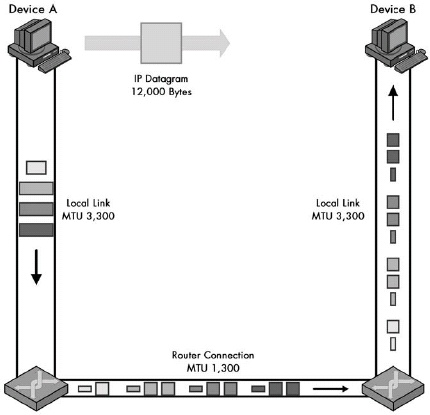
\includegraphics[width=.7\textwidth]{images/ipv4-datagram-fragmentation.jpg}
   \caption
      [IPv4 datagram fragmentation]
      {IPv4 datagram fragmentation --
      This example illustrates a two-step fragmentation of a large IP datagram.
      The boxes represent datagrams or datagram fragments and are shown to scale.
      The original datagram is 12,000 bytes, represented by the large, gray box.
      To transmit this data over the first local link, device A splits it into four fragments, shown on the left.
      The first router must fragment each of these into smaller fragments to send them over the 1,300-byte MTU link, as shown on the bottom.
      Note that the second router does not reassemble the 1,300-byte fragments, even though its link to device B has an MTU of 3,300 bytes.
      (\Vref{sec:ip-fragmentation-process} describes the process by which the fragments in this example are created.)}
   \label{fig:ipv4-datagram-fragmentation}
\end{figure}



\section{Internet minimum MTU: 576 bytes}

Routers are required to handle an MTU of at least 576 bytes.
This value is specified in RFC 791; it was chosen to allow a data block of at least 512 bytes, plus room for the standard IP header and options.
Since this is the minimum size specified in the IP standard, 576 bytes has become a common default MTU value used for IP datagrams.
Even if a host is connected over a local network with an MTU larger than 576 bytes,
it may choose to use an MTU value of 576 to ensure that no further fragmentation will be required by intermediate routers.

\begin{note}
While intermediate routers may further fragment an already-fragmented IP message, they do not reassemble fragments.
Reassembly is done only by the recipient device.
This has some advantages and some disadvantages, as we will see when we examine the reassembly process in the ``IP Message Reassembly'' section later in this
chapter.
\end{note}



\section{MTU path discovery}

When we're trying to send a great deal of data, efficiency in message transmissions becomes important.
The larger the IP datagram we send, the smaller the percentage of bytes wasted for overhead such as header fields.
This means that, ideally, we want to use the largest MTU possible without requiring fragmentation for its transmission.

To determine the optimal MTU to use for a route between two devices, we
would need to know the MTU of every link on that route -- information that the endpoints of the connection simply don't have.
However, the connection endpoint can determine the MTU of the overall route by using
\emph{MTU path discovery},\index{MTU path discovery} which uses an error-reporting mechanism built into ICMP.

One of the message types defined in ICMP version 4 (ICMPv4) is the
Destination Unreachable message (see \protect\hyperlink{ch32.html}{Chapter~32}),
which is returned under various conditions where an IP datagram cannot
be delivered. One of these situations is when a datagram is too large to
be forwarded by a router over a physical link, but this datagram has its
Don't Fragment (DF) flag set to prevent fragmentation. In this case, the
datagram must be discarded and a Destination Unreachable message sent
back to the source. A device can exploit this capability by testing the
path with datagrams of different sizes, to see how large they must be
before they are rejected.

The source node typically sends a datagram that has the MTU of its local
physical link, since that represents an upper bound for any path to or
from that device. If this datagram goes through without any errors, the
device knows it can use that value for future datagrams to that
destination. If it gets back any Destination Unreachable - Fragmentation
Needed and DF Set messages, it knows that a link between it and the
destination has a smaller MTU. It tries again using a smaller datagram
size, and it continues until it finds the largest MTU that can be used
on the path.


As explained in the previous section, when an IP datagram is too large
for the MTU of the underlying data link layer technology used for the
next leg of its journey, it must be fragmented before it can be sent
across the network. The higher-layer message to be transmitted is not
sent in a single IP datagram, but rather broken down into fragments that
are sent separately. In some cases, the fragments themselves may need to
be fragmented further.

Fragmentation is key to implementing a network-layer internetwork that is independent
of lower-layer details, but it introduces significant complexity to IP.
Remember that IP is an unreliable, connectionless protocol. IP datagrams
can take any of several routes on their way from the source to the
destination, and some may not even make it to the destination at all.
When a message is fragmented, this converts a single datagram into many,
which introduces several new concerns:

\begin{description}
   \item[Sequencing and placement]
      The fragments will typically be sent in sequential order from the beginning of the message to the end,
      but they won't necessarily show up in the order in which they were sent.
      The receiving device must be able to determine the sequence of the fragments to reassemble them in the correct order.
      In fact, some implementations send the last fragment first, so the receiving device will immediately know the full size of the original, complete datagram.
      This makes keeping track of the order of segments even more essential.

   \item[Separation of fragmented messages]
      A source device may need to send more than one fragmented message at a time, or it may send multiple datagrams that are fragmented en route.
      This means that the destination may be receiving multiple sets of fragments that must be put back together.
      Imagine a box containing pieces from two, three, or more jigsaw puzzles, and you understand this issue.

   \item[Completion]
      The destination device must be able to tell when it has received all of the fragments so it knows when to start reassembly
      (or when to give up if it didn't get all the pieces).
\end{description}

To address these concerns and allow the proper reassembly of the fragmented message,
IP includes several fields in the IP format header that convey information from the source to the destination about the fragments.
Some of these fields contain a common value for all the fragments of the message; others are different for each fragment.




\section{The IP fragmentation process}
\label{sec:ip-fragmentation-process}

The device performing the fragmentation follows a specific algorithm to divide the message into fragments for transmission.
The exact implementation of the
fragmentation process depends on the device. For example, consider an IP
message 12,000 bytes wide (including the 20-byte IP header) that needs
to be sent over a link with an MTU of 3,300 bytes.
\Cref{fig:ipv4-datagram-fragmentation-process} depicts a typical method by which this fragmentation might be performed.


\begin{figure}
   \centering
   %\includegraphics{httpatomoreillycomsourcenostarchimages287861.png.jpg}
   \caption
      [IPv4 datagram fragmentation process]
      {IPv4 datagram fragmentation process -- In this diagram, the MF and Fragment Offset fields of each fragment are shown for reference.
      The Data fields are shown to scale (the length of each is proportional to the number of bytes in the fragment).}
   \label{fig:ipv4-datagram-fragmentation-process}
\end{figure}


The four fragments shown in \cref{fig:ipv4-datagram-fragmentation-process} are created as follows:

\begin{itemize}
   \item
      The first fragment is created by taking the first 3,300 bytes of the 12,000-byte IP datagram.
      This includes the original header, which becomes the IP header of the first fragment (with certain fields changed, as described in the next section).
      So, 3,280 bytes of data are in the first fragment.
      This leaves 8,700 bytes ($11980-3280$) to encapsulate.
   \item
      The next 3280 bytes of data are taken from the 8700~bytes that remain after
      the first fragment is built and paired with a new header to create the second fragment.
      This leaves 5420 bytes.
   \item
      The third fragment is created from the next 3280 bytes of data, with a 20-byte header. This leaves 2140 bytes of data.
   \item
      The remaining 2140 bytes are placed into the fourth fragment, with a 20-byte header.
\end{itemize}

There are two important points here. First, IP fragmentation does \emph{not} work by fully encapsulating the original IP message into the Data fields of the fragments.
If this were the case, the first 20~bytes of the Data field of the first fragment would contain the original
IP header.
(This technique is used by some other protocols, such as the PPP Multilink Protocol.)
The original IP header is transformed into the IP header of the first fragment.

Second, note that the total number of bytes transmitted increases: we are sending 12,060 bytes ($3300\times 3 + 2160$), instead of 12,000 bytes.
The extra 60 bytes are from the additional headers in the second, third, and fourth fragments.
(The increase in size could theoretically be even larger if the headers contain options.)



\section{Fragmentation-related IP datagram header fields}

\protect\hypertarget{ch22s02.htmlux5cux23idx-CHP-22-0809}{}{}When a
sending device or router fragments a datagram, it must provide
information that will allow the receiving device to identify the
fragments and reassemble them into the original datagram. This
information is recorded by the fragmenting device in a number of fields
in the IP datagram header:

\begin{description}
   \item[Total length]
      After fragmenting, the Total Length field indicates the length of each fragment, not the length of the overall message.
      Normally, the fragment size is selected to match the MTU value in bytes.
      However, fragments must have a length that is a multiple of 8, to allow proper offset specification (handled by the Fragment Offset field).
      The last fragment will usually be shorter than the others because it will contain a leftover piece, unless the message length happens to be an exact multiple of the fragment size.

   \item[Identification]
      To solve the problem of pieces from many
jigsaw puzzles in the same box, a unique identifier is assigned to each
message being fragmented. This is like writing a different number on the
bottom of each piece of a jigsaw puzzle before tossing it in the box.
This value is placed in the Identification field in the IP header of
each fragment sent. The Identification field is 16 bits wide, so a total
of 65,536 different identifiers can be used. Obviously, we want to make
sure that each message that is being fragmented for delivery has a
different identifier. The source can decide how it generates unique
identifiers. This may be done through something as simple as a counter
that is incremented each time a new set of fragments is created.

   \item[More fragments]
      The More Fragments flag is set to a 1 for all fragments except the last one, which has it set to 0. When the fragment with a
value of 0 in the More Fragments flag is seen, the destination knows it
has received the last fragment of the message.

   \item[Fragment offset]
      The Fragment Offset field solves the problem
of sequencing fragments by indicating to the recipient device where in
the overall message each particular fragment should be placed. The field
is 13 bits wide, so the offset can be from 0 to 8,191. Fragments are
specified in units of 8 bytes, which is why fragment length must be a multiple of eight.
Uncoincidentally, $8191\times 8$ is 65,528, just about the maximum size allowed for an IP datagram.
In the example shown in \protect\hyperlink{ch22s02.htmlux5cux23ipv4_datagram_fragmentation_process_in_t}{Figure~22-3},
the first fragment would have a Fragment Offset of 0, the second would have an offset of 410 (3,280/8), the third would have an offset of 820
(6,560/8), and the fourth would have an offset of 1,230.
\end{description}

An IP datagram has a couple of other fields related to fragmentation.
First, if a datagram containing options must be fragmented, some of the
options may be copied to each of the fragments. This is controlled by
the \protect\hypertarget{ch22s02.htmlux5cux23idx-CHP-22-0812}{}{}Copied
flag in each option field.

Second, in the IP header, there is a flag called
\protect\hypertarget{ch22s02.htmlux5cux23idx-CHP-22-0813}{}{}Don't
Fragment. This field can be set to 1 by a transmitting device to specify
that a datagram should not be fragmented in transit. This may be used in
certain circumstances where the entire message must be delivered intact
for some reason. It may also be used if the destination device has a
limited IP implementation and cannot reassemble fragments, and it is
also used for testing the MTU of a link. Normally, however, devices
don't care about fragmentation, and this field is left at 0.

If a router encounters a datagram too large to pass over the next
physical network but with the Don't Fragment bit set to 1, it cannot
fragment the datagram and it cannot pass it along either, so it is
stuck. It will generally drop the datagram and return an ICMP
Destination Unreachable error message: ``Fragmentation Needed and Don't
Fragment Bit Set.'' This is used in MTU path discovery, as described
earlier in this chapter.

\begin{keyconcept}
When an MTU requirement forces a datagram to be
fragmented, it is split into several smaller IP datagrams, each
containing part of the original. The header of the original datagram is
changed into the header of the first fragment, and new headers are
created for the other fragments. Each is set to the same Identification
value to mark them as part of the same original datagram. The Fragment
Offset of each is set to the location where the fragment belongs in the
original. The More Fragments field is set to 1 for all fragments but the
last, to let the recipient know when it has received all the fragments.
\end{keyconcept}

When a datagram is fragmented, it becomes multiple fragment datagrams. The
destination of the overall message must collect these fragments and
reassemble them into the original message.

While reassembly is the complement to fragmentation, the two processes are not symmetric.
A primary differentiation between the two is that intermediate routers
can fragment a single datagram or further fragment a datagram that is
already a fragment, but intermediate devices do not perform reassembly;
reassembly happens only at the message's ultimate destination. Thus, if
a datagram at an intermediate router on one side of a physical network
with an MTU of 1,300 bytes causes fragmentation of a 3,300-byte
datagram, the router on the other end of this 1,300 MTU link will
\emph{not} restore the 3,300-byte datagram to its original state. It
will send all the 1,300-byte fragments on down the internetwork, as
shown in
\protect\hyperlink{ch22.htmlux5cux23ipv4_datagram_fragmentation_this_example}{Figure~22-2},
earlier in the chapter.

In IP version 4 (IPv4), fragmentation can be performed by a router
between the source and destination of an IP datagram, but reassembly is
done only by the destination device.

There are a number of reasons why the decision was made to implement IP
reassembly this way. Perhaps the most important reason is that fragments
can take different routes to get from the source to destination, so any
given router may not see all the fragments in a message. Another reason
is that if routers needed to worry about reassembling fragments, their
complexity would increase. Finally, reassembly of a message requires
that we wait for all fragments before sending on the reassembled
message. Having routers do this would slow down routing. Since routers
don't reassemble messages, they can immediately forward all fragments on
to the ultimate recipient.

However, there are drawbacks to this design as well. One is that it
results in more, smaller fragments traveling over longer routes than if
intermediate reassembly occurred. This increases the chances of a
fragment getting lost and the entire message being discarded. Another is
a potential inefficiency in the utilization of data link layer frame
capacity. In the example of a 3,300-byte datagram being fragmented for a
1,300-byte MTU link, the 1,300-byte fragments would not be reassembled
back into a 3,300-byte datagram at the end of the 1,300-MTU link. If the
next link after that one also had an MTU of 3,300 bytes, we would need
to send three frames, each encapsulating a 1,300-byte fragment, instead
of a single larger frame, which is slightly slower.

As described in the previous section, several IP header fields are
filled in when a message is fragmented to give the receiving device the
information it requires to properly reassemble the fragments. The
receiving device follows a procedure to keep track of the fragments as
they are received and build up its copy of the total received message
from the source device. Most of its efforts are geared toward dealing
with the potential difficulties associated with IP being an unreliable
protocol.

The details of implementation of the reassembly process are specific to each device, but reassembly generally includes the following functions:
\begin{description}
\item[Fragment recognition and fragmented message identification]
   The recipient knows it has received a message fragment the first time it sees a datagram with the More Fragments bit set to 1 or the Fragment
Offset a value other than 0.
It identifies the message based on the source and destination IP addresses, the protocol specified in the
header, and the Identification field generated by the sender.

\item[Buffer initialization]
The receiving device initializes a buffer where it can store the fragments of the message as they are
received. It keeps track of which portions of this buffer have been
filled with received fragments, perhaps using a special table. By doing
this, it knows when the buffer is partially filled with received
fragments and when it is completely full.

\item[Timer initialization]
The receiving device sets up a timer for
reassembly of the message. Since it is possible that some fragments may
never show up, this timer ensures that the device will not wait an
infinite time trying to reassemble the message.

\item[Fragment receipt and processing]
Whenever a fragment of this message arrives (as indicated by it having the same source and
destination addresses, protocol, and Identification as the first
fragment), the fragment is processed. It is inserted into the message
buffer in the location indicated by its Fragment Offset field. The
device also makes note of the fact that this portion of the message has
been received.
\end{description}

Reassembly is complete when the entire buffer has been filled and the
fragment with the More Fragments bit set to 0 is received, indicating
that it is the last fragment of the datagram. The reassembled datagram
is then processed in the same way as a normal, unfragmented datagram. On
the other hand, if the timer for the reassembly expires with any of the
fragments missing, the message cannot be reconstructed. The fragments
are discarded, and an ICMP Time Exceeded message is generated. Since IP
is unreliable, it relies on higher-layer protocols such as the
Transmission Control Protocol (TCP) to determine that the message was
not properly received and then retransmit it.

